\documentclass[sigconf,nonacm]{acmart}

\setcopyright{none}
\settopmatter{printacmref=false}
\renewcommand\footnotetextcopyrightpermission[1]{}
\pagestyle{plain}

\usepackage{booktabs}
\usepackage{tabularx}
\usepackage{multirow}
\usepackage{amsmath}
\let\Bbbk\relax
\usepackage{amssymb}
\usepackage{tikz}
\usepackage{pgfplots}
\pgfplotsset{compat=1.18}
\usepackage{url}
\urlstyle{rm}

\usetikzlibrary{arrows.meta,positioning,calc,shapes.geometric,
                decorations.pathreplacing,patterns}

%% ── colour palette ───────────────────────────────────────────────────────────
\definecolor{cconf}{RGB}{ 50,110,190}   % Confidentiality — blue
\definecolor{cintg}{RGB}{ 40,150, 70}   % Integrity — green
\definecolor{cavail}{RGB}{200,100, 30}  % Availability — orange
\definecolor{cred} {RGB}{200, 50, 50}   % Violation / risk
\definecolor{cyel} {RGB}{190,165,  0}   % Warning
\definecolor{cgrn} {RGB}{ 40,150, 70}   % Safe / compliant
\definecolor{cgry} {RGB}{100,100,100}   % Neutral
\definecolor{cblu} {RGB}{ 50,110,190}   % Blue accent

\begin{CCSXML}
<ccs2012>
  <concept>
    <concept_id>10002978.10003006</concept_id>
    <concept_desc>Security and privacy~Systems security</concept_desc>
    <concept_significance>500</concept_significance>
  </concept>
  <concept>
    <concept_id>10002978.10003022</concept_id>
    <concept_desc>Security and privacy~Privacy-preserving protocols</concept_desc>
    <concept_significance>300</concept_significance>
  </concept>
  <concept>
    <concept_id>10011007.10011006.10011050.10011017</concept_id>
    <concept_desc>Software and its engineering~Cloud computing</concept_desc>
    <concept_significance>300</concept_significance>
  </concept>
</ccs2012>
\end{CCSXML}

\ccsdesc[500]{Security and privacy~Systems security}
\ccsdesc[300]{Security and privacy~Privacy-preserving protocols}

\title{Government Efficiency vs.\ Cybersecurity: A CIA Triad Analysis of the DOGE Social Security Data Incident}

\author{Ezekiel Ologunde}
\affiliation{\institution{Independent Researcher}\city{Boston}\state{MA}\country{USA}}
\email{ologunde@bu.edu}

\begin{abstract}
The Department of Government Efficiency's (DOGE) handling of Social Security
Administration data in 2025 represents a critical case study in the tension between
operational efficiency and cybersecurity architecture principles. This paper analyzes
DOGE's approach through the lens of the CIA triad---Confidentiality, Integrity, and
Availability---to understand how the pursuit of rapid fraud detection compromised
fundamental security principles. The incident, involving the transfer of over 300 million
Americans' personally identifiable information to an unsecured cloud environment,
demonstrates systemic failures in implementing established cybersecurity frameworks.
Through examination of existing government security standards and comparison with
historical data breaches, this analysis reveals the critical importance of integrating
security architecture from inception rather than treating it as a post-implementation
consideration. The findings suggest that with proper implementation of zero trust
architecture, risk-based security controls, and adherence to established frameworks like
FISMA and NIST guidelines, government agencies can achieve both mission effectiveness
and robust data protection.
\end{abstract}

\keywords{cybersecurity architecture, CIA triad, zero trust, government data security,
FISMA compliance, DOGE, Social Security Administration, PII protection}

\begin{document}
\hfuzz=5pt
\maketitle

%%─────────────────────────────────────────────────────────────────────────────
\section{Introduction}
%%─────────────────────────────────────────────────────────────────────────────

The intersection of government efficiency initiatives and cybersecurity requirements
presents one of the most challenging aspects of modern public administration. In 2025,
the newly formed Department of Government Efficiency (DOGE) undertook an ambitious
mission to identify fraudulent Social Security payments---a laudable operational goal.
However, their approach to handling sensitive citizen data violated fundamental
cybersecurity architecture principles, creating what cybersecurity expert Charles Borges
described as ``serious data security lapses'' that put over 300 million Americans at
risk~\cite{nazzaro2025}.

DOGE copied the entire NUMIDENT database---containing Social Security numbers,
birthdates, addresses, and other personally identifiable information (PII)---to an
unsecured cloud environment with no verified oversight~\cite{nazzaro2025}. This action
represents a systematic violation of the CIA triad principles that form the foundation
of modern cybersecurity architecture.

The significance of this case extends beyond a single policy misstep. It illuminates
the broader challenge facing government agencies attempting to modernize operations
while maintaining security posture in an increasingly complex threat landscape. As
government services become more digital and analytical, the tension between
speed-to-value and security compliance becomes more pronounced, requiring sophisticated
architectural solutions rather than binary trade-offs.

\subsection{Research Contributions}

\begin{itemize}
  \item Systematic CIA triad analysis of the DOGE NUMIDENT data transfer incident,
        identifying specific control failures across all three security pillars
  \item Comparison with the 2015 OPM breach to identify recurring patterns of federal
        cybersecurity governance failure
  \item Quantified trade-off analysis for large-scale government analytics environments
  \item Concrete zero trust and DevSecOps implementation guidance for government
        analytics use cases
  \item Policy recommendations addressing institutional, technical, and governance gaps
\end{itemize}

%%─────────────────────────────────────────────────────────────────────────────
\section{The CIA Triad in Government Cybersecurity}
%%─────────────────────────────────────────────────────────────────────────────

\subsection{Foundational Principles}

The CIA triad---Confidentiality, Integrity, and Availability---represents the cornerstone
of information security and serves as the fundamental framework for evaluating
cybersecurity architecture decisions. Figure~\ref{fig:cia_triad} illustrates the
three pillars and their interdependencies.

\begin{figure}[h]
\centering
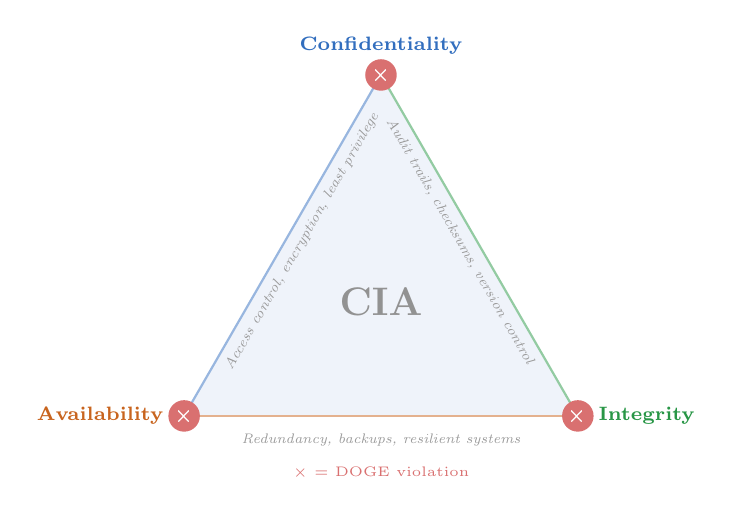
\begin{tikzpicture}[
  font=\fontsize{6.5pt}{8pt}\selectfont,
  >=Stealth
]
  %% Equilateral triangle, side 5 cm
  \def\s{5.0}
  \coordinate (C) at (0,        {sqrt(3)/2*\s});  % Confidentiality apex
  \coordinate (A) at ({-\s/2},  0);               % Availability bottom-left
  \coordinate (I) at ({ \s/2},  0);               % Integrity  bottom-right

  %% Filled triangle
  \fill[cconf!8] (C)--(A)--(I)--cycle;
  \draw[thick, cconf!50] (C)--(A);
  \draw[thick, cintg!50] (I)--(C);
  \draw[thick, cavail!50] (A)--(I);

  %% Central label
  \node[font=\fontsize{14pt}{17pt}\selectfont\bfseries, text=cgry!70]
    at (0, {sqrt(3)/6*\s}) {CIA};

  %% Vertex labels
  \node[above=4pt, font=\fontsize{7pt}{9pt}\selectfont\bfseries, text=cconf]
    at (C) {Confidentiality};
  \node[left=4pt, font=\fontsize{7pt}{9pt}\selectfont\bfseries, text=cavail,
        align=center] at (A) {Availability};
  \node[right=4pt, font=\fontsize{7pt}{9pt}\selectfont\bfseries, text=cintg,
        align=center] at (I) {Integrity};

  %% Edge annotations
  \node[font=\fontsize{5.5pt}{7pt}\selectfont\itshape, text=cgry!65,
        rotate=60] at (-1.0, {sqrt(3)/4*\s+0.05})
    {Access control, encryption, least privilege};
  \node[font=\fontsize{5.5pt}{7pt}\selectfont\itshape, text=cgry!65,
        rotate=-60] at ( 1.0, {sqrt(3)/4*\s+0.05})
    {Audit trails, checksums, version control};
  \node[font=\fontsize{5.5pt}{7pt}\selectfont\itshape, text=cgry!65]
    at (0, -0.30) {Redundancy, backups, resilient systems};

  %% DOGE violation markers on each vertex
  \node[circle, fill=cred!70, minimum size=0.40cm, inner sep=0pt,
        font=\fontsize{6pt}{7.5pt}\selectfont\bfseries, text=white]
    at (C) {\texttimes};
  \node[circle, fill=cred!70, minimum size=0.40cm, inner sep=0pt,
        font=\fontsize{6pt}{7.5pt}\selectfont\bfseries, text=white]
    at (A) {\texttimes};
  \node[circle, fill=cred!70, minimum size=0.40cm, inner sep=0pt,
        font=\fontsize{6pt}{7.5pt}\selectfont\bfseries, text=white]
    at (I) {\texttimes};

  \node[font=\fontsize{5.5pt}{7pt}\selectfont, text=cred!70]
    at (0, -0.72) {$\times$ = DOGE violation};
\end{tikzpicture}
\caption{The CIA triad with DOGE violation markers (red $\times$) at all three
  vertices. Each edge lists the primary controls linking the two adjacent pillars.
  DOGE's NUMIDENT transfer violated all three simultaneously.}
\label{fig:cia_triad}
\end{figure}

In the context of government operations, these principles take on heightened importance
due to the sensitivity of citizen data and potential national security implications.
NIST SP~800-207 specifies that zero trust architecture ensures ``authentication and
authorization are continual processes rather than one-time events''~\cite{nist800207}.
The Federal Information Security Modernization Act (FISMA) establishes legal
requirements for agencies to implement comprehensive security controls~\cite{cms2025}.

\subsection{Historical Context: The OPM Breach Precedent}

The 2015 Office of Personnel Management (OPM) breach serves as a directly relevant
precedent: millions of SF-86 background investigation forms and fingerprint records
were compromised due to inadequate security controls~\cite{fruhlinger2020}. The
parallels to DOGE are striking---both incidents involved large-scale data transfers
without proper security oversight; both prioritized operational convenience over
established security protocols; and both ignored fundamental data protection
architecture principles. The lessons from OPM were clear, yet DOGE's approach
suggests these lessons were not internalized across the federal government, highlighting
systemic failures in cybersecurity culture and governance.

%%─────────────────────────────────────────────────────────────────────────────
\section{DOGE's CIA Triad Violations}
%%─────────────────────────────────────────────────────────────────────────────

Figure~\ref{fig:violations} maps the specific control failures across the three CIA
triad pillars.

\begin{figure}[h]
\centering
\resizebox{\columnwidth}{!}{%
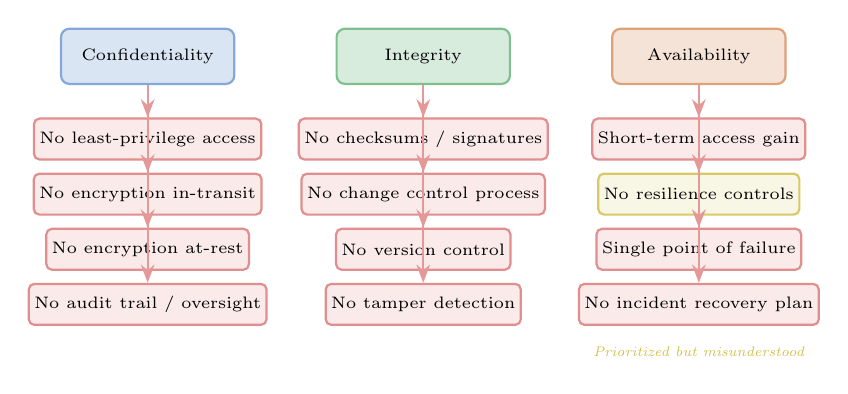
\begin{tikzpicture}[
  font=\fontsize{6.5pt}{8pt}\selectfont,
  >=Stealth,
  pillar/.style={rectangle, rounded corners=3pt, draw, thick,
                 minimum width=2.2cm, minimum height=0.70cm,
                 text centered, inner sep=3pt},
  fail/.style={rectangle, rounded corners=2pt, draw=cred!55, thick,
               fill=cred!10, minimum width=2.0cm, minimum height=0.52cm,
               text centered, font=\fontsize{6pt}{7.5pt}\selectfont, inner sep=2pt},
  arr/.style={-{Stealth}, thick, cgry!55}
]
  %% Three pillar headers
  \node[pillar, fill=cconf!18, draw=cconf!60] (P1) at (0,    0) {Confidentiality};
  \node[pillar, fill=cintg!18, draw=cintg!60] (P2) at (3.5,  0) {Integrity};
  \node[pillar, fill=cavail!18,draw=cavail!60] (P3) at (7.0,  0) {Availability};

  %% Confidentiality failures
  \node[fail] (f11) at (0,  -1.05) {No least-privilege access};
  \node[fail] (f12) at (0,  -1.75) {No encryption in-transit};
  \node[fail] (f13) at (0,  -2.45) {No encryption at-rest};
  \node[fail] (f14) at (0,  -3.15) {No audit trail / oversight};

  %% Integrity failures
  \node[fail] (f21) at (3.5,-1.05) {No checksums / signatures};
  \node[fail] (f22) at (3.5,-1.75) {No change control process};
  \node[fail] (f23) at (3.5,-2.45) {No version control};
  \node[fail] (f24) at (3.5,-3.15) {No tamper detection};

  %% Availability failure
  \node[fail] (f31) at (7.0,-1.05) {Short-term access gain};
  \node[fail, draw=cyel!60, fill=cyel!10] (f32) at (7.0,-1.75) {No resilience controls};
  \node[fail] (f33) at (7.0,-2.45) {Single point of failure};
  \node[fail] (f34) at (7.0,-3.15) {No incident recovery plan};

  \foreach \f in {f11,f12,f13,f14}
    \draw[arr, cred!50] (P1.south) -- (\f.north);
  \foreach \f in {f21,f22,f23,f24}
    \draw[arr, cred!50] (P2.south) -- (\f.north);
  \foreach \f in {f31,f32,f33,f34}
    \draw[arr, cred!50] (P3.south) -- (\f.north);

  %% "Paradox" annotation for availability
  \node[font=\fontsize{5.5pt}{7pt}\selectfont\itshape, text=cyel!70]
    at (7.0,-3.75) {Prioritized but misunderstood};
\end{tikzpicture}
}%
\caption{DOGE CIA triad control failures. Availability (orange) is marked as
  ``paradox'': DOGE prioritized immediate data access but misunderstood availability
  as unrestricted access rather than resilient, controlled availability.}
\label{fig:violations}
\end{figure}

\subsection{Confidentiality Failures}

DOGE's transfer of the entire NUMIDENT database to an unsecured cloud environment with
no verified oversight represents a fundamental breach of confidentiality
protocols~\cite{nazzaro2025}.

\textbf{Access Control.} Granting blanket administrative access to DOGE officials
violated the principle of least privilege. NIST SP~800-207 explicitly requires that
``there is no implicit trust granted to assets or user accounts based solely on their
physical or network location''~\cite{nist800207}, yet DOGE's approach granted broad
access based purely on organizational affiliation.

\textbf{Encryption Deficiencies.} The available complaint evidence provides no
indication of encryption-in-transit or encryption-at-rest protections. Modern
cybersecurity architecture requires cryptographic controls throughout data lifecycle,
particularly in cloud environments.

\textbf{Monitoring and Audit Gaps.} The complete absence of oversight mechanisms meant
that unauthorized access or data manipulation could occur without detection, fundamentally
undermining the confidentiality assurance that citizens expect from government
data handling.

\subsection{Integrity Compromises}

Without proper logging and monitoring, there was no way to verify whether data had been
altered, corrupted, or manipulated during transfer or processing. The absence of
checksums, digital signatures, change management, and version control left the system
vulnerable to both accidental corruption and malicious manipulation---a ``dangerously
high-risk gamble'' in the words of cybersecurity expert Charles Borges~\cite{nazzaro2025}.

\subsection{Availability Paradox}

Ironically, availability was the one pillar DOGE arguably prioritized, though their
approach ultimately undermined long-term availability assurance. By creating a separate
cloud environment optimized for fraud detection analytics, they may have initially
improved data accessibility for their specific mission. However, true availability in
cybersecurity architecture means ensuring that \emph{authorized} users can access
systems when needed, while maintaining security controls that prevent unauthorized
access or system compromise. DOGE's approach provided immediate access but created
substantial risks that could have led to complete system unavailability in the event
of a breach.

%%─────────────────────────────────────────────────────────────────────────────
\section{Trade-offs in Large-Scale Government Analytics}
%%─────────────────────────────────────────────────────────────────────────────

\subsection{Performance versus Security}

Processing massive government datasets for fraud detection requires careful consideration
of competing priorities. As Morris notes, ``prioritizing one element of the CIA triad
almost always impacts the others,'' creating complex trade-offs that require
sophisticated architectural solutions~\cite{morris2023}. Encryption, access controls,
and audit logging all introduce computational overhead; but this overhead must be
weighed against the cost of a breach affecting 300 million citizens.

\subsection{Centralization versus Distribution}

Table~\ref{tab:tradeoffs} summarizes the architectural trade-offs that DOGE faced.
Centralization enables sophisticated cross-referencing and machine learning approaches
that improve fraud detection. However, it also creates a single point of failure and
dramatically amplifies the potential impact of any breach. By centralizing data without
centralizing security oversight, DOGE achieved the worst of both architectural
approaches.

\begin{table}[h]
\caption{Centralization vs.\ Distribution Trade-offs for Government Analytics.}
\label{tab:tradeoffs}
\small
\begin{tabularx}{\columnwidth}{@{}p{2.1cm}X X@{}}
\toprule
\textbf{Dimension} & \textbf{Centralized (DOGE approach)} & \textbf{Distributed / Secure} \\
\midrule
Analytics power & High ML/cross-referencing capability & Moderate (federated) \\
Breach impact   & All 300M records exposed             & Limited blast radius \\
Governance      & Single control point (if secured)    & Complex but resilient \\
Audit surface   & Smaller (if logged)                  & Distributed logs required \\
Compliance      & Easier when properly designed        & Requires coordination \\
DOGE outcome    & Centralized data, decentralized security & Neither benefit achieved \\
\bottomrule
\end{tabularx}
\end{table}

%%─────────────────────────────────────────────────────────────────────────────
\section{Cybersecurity Architecture Solutions}
%%─────────────────────────────────────────────────────────────────────────────

\subsection{Zero Trust Implementation}

Zero trust architecture represents ``an evolving set of cybersecurity paradigms that
move defenses from static, network-based perimeters to focus on users, assets, and
resources''~\cite{nist2021zt}. Figure~\ref{fig:zt_model} illustrates a zero trust
model for government analytics that could have prevented DOGE's failures.

\begin{figure}[h]
\centering
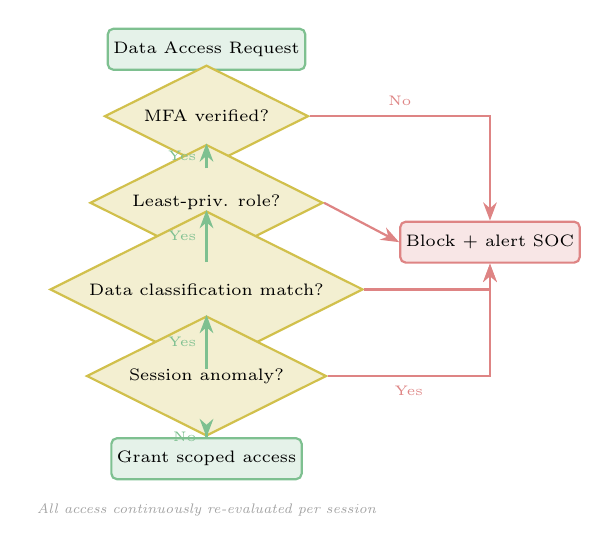
\begin{tikzpicture}[
  font=\fontsize{6.5pt}{8pt}\selectfont,
  >=Stealth,
  dec/.style={diamond, draw=cyel!70, thick, fill=cyel!18, aspect=2.0,
              minimum width=2.2cm, minimum height=0.72cm,
              text centered, font=\fontsize{6pt}{7.5pt}\selectfont},
  yes/.style={rectangle, rounded corners=2pt, draw=cgrn!60, thick,
              fill=cgrn!12, minimum width=1.9cm, minimum height=0.52cm,
              text centered, font=\fontsize{6pt}{7.5pt}\selectfont, inner sep=2pt},
  no/.style={rectangle, rounded corners=2pt, draw=cred!60, thick,
             fill=cred!12, minimum width=1.9cm, minimum height=0.52cm,
             text centered, font=\fontsize{6pt}{7.5pt}\selectfont, inner sep=2pt},
  arr/.style={-{Stealth}, thick}
]
  \node[yes, minimum width=2.4cm] (req) at (0, 0.65)
    {Data Access Request};
  \draw[-{Stealth}, cblu!50, thick] (req.south)--(0,0.13);

  \node[dec] (d1) at (0, -0.20) {MFA verified?};
  \node[dec] (d2) at (0, -1.30) {Least-priv. role?};
  \node[dec] (d3) at (0, -2.40) {Data classification match?};
  \node[dec] (d4) at (0, -3.50) {Session anomaly?};
  \node[yes] (ok) at (0, -4.55) {Grant scoped access};

  \node[no] (bk) at (3.6,-1.80) {Block + alert SOC};

  \draw[arr, cgrn!60] (d1.south)--node[left,font=\fontsize{5.5pt}{7pt}\selectfont]{Yes}(d2.north);
  \draw[arr, cgrn!60] (d2.south)--node[left,font=\fontsize{5.5pt}{7pt}\selectfont]{Yes}(d3.north);
  \draw[arr, cgrn!60] (d3.south)--node[left,font=\fontsize{5.5pt}{7pt}\selectfont]{Yes}(d4.north);
  \draw[arr, cgrn!60] (d4.south)--node[left,font=\fontsize{5.5pt}{7pt}\selectfont]{No}(ok.north);

  \draw[arr, cred!60] (d1.east)--node[above,font=\fontsize{5.5pt}{7pt}\selectfont]{No}(3.6,-0.20)--(bk.north);
  \draw[arr, cred!60] (d2.east)--(bk.west);
  \draw[arr, cred!60] (d3.east)--(3.6,-2.40)--(bk.south);
  \draw[arr, cred!60] (d4.east)--node[below,font=\fontsize{5.5pt}{7pt}\selectfont]{Yes}(3.6,-3.50)--(bk.south);

  \node[font=\fontsize{5.5pt}{7pt}\selectfont\itshape, text=cgry!60]
    at (0,-5.20) {All access continuously re-evaluated per session};
\end{tikzpicture}
\caption{Zero trust access evaluation model for government analytics. Every request
  is validated against MFA, least-privilege role, data classification alignment, and
  real-time anomaly detection before scoped access is granted.}
\label{fig:zt_model}
\end{figure}

For DOGE's specific use case, proper zero trust implementation would have provided:
\textbf{continuous authentication} instead of blanket administrative grants;
\textbf{micro-segmentation} allowing analysts to access only the specific data fields
needed for fraud detection rather than copying entire databases; and \textbf{policy-based
access control} with dynamic policies based on user role, device posture, and data
sensitivity~\cite{nist180035}.

\subsection{Risk-Based Security Controls}

Government agencies should implement graduated security controls based on data
sensitivity. The NUMIDENT database clearly requires maximum protection levels, yet
DOGE treated it as routine operational data. Table~\ref{tab:controls} maps recommended
controls to the three CIA triad pillars.

\begin{table}[h]
\sloppy
\caption{Risk-Based Controls Mapped to CIA Triad Pillars.}
\label{tab:controls}
\small
\begin{tabularx}{\columnwidth}{@{}p{2.4cm}X p{1.1cm}@{}}
\toprule
\textbf{Pillar} & \textbf{Required Control} & \textbf{DOGE Status} \\
\midrule
\multirow{3}{*}{Confidentiality} & Least-privilege access & Absent \\
 & AES-256 encryption (transit + rest) & Absent \\
 & Continuous audit logging & Absent \\
\addlinespace[2pt]
\multirow{3}{*}{Integrity} & Cryptographic checksums & Absent \\
 & Change management / version control & Absent \\
 & Tamper-evident logging & Absent \\
\addlinespace[2pt]
\multirow{3}{*}{Availability} & Redundant systems / failover & Absent \\
 & Tested recovery procedures & Absent \\
 & Resilience monitoring & Absent \\
\bottomrule
\end{tabularx}
\end{table}

\subsection{DevSecOps Integration}

Modern cybersecurity architecture emphasizes integrating security throughout the
development and deployment lifecycle rather than treating it as an afterthought:

\textbf{Security by Design.} Building security controls into the architecture from the
beginning is more effective and less costly than retrofitting measures after deployment.

\textbf{Automated Security Testing.} Continuous security testing throughout the
development process can identify vulnerabilities before they reach production
environments.

\textbf{Infrastructure as Code (IaC).} Managing infrastructure through code enables
consistent application of security policies and makes it easier to audit and verify
security controls---directly addressing the undocumented configuration changes that
occurred in DOGE's environment.

%%─────────────────────────────────────────────────────────────────────────────
\section{Regulatory and Compliance Implications}
%%─────────────────────────────────────────────────────────────────────────────

\subsection{FISMA Compliance Failures}

FISMA defines a comprehensive framework to protect government information, operations,
and assets~\cite{upguard2025}. Figure~\ref{fig:compliance} maps DOGE's actions against
FISMA requirements.

\begin{figure}[h]
\centering
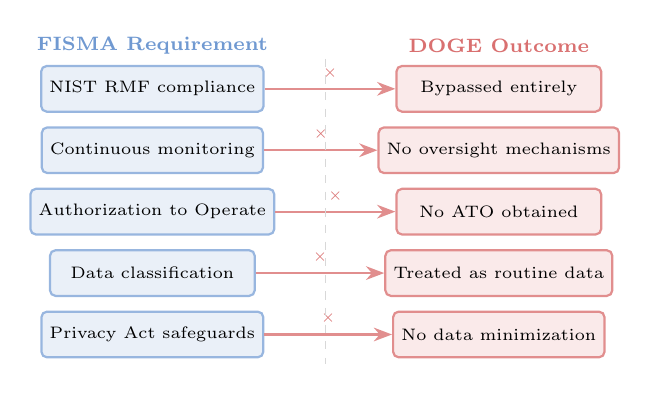
\begin{tikzpicture}[
  font=\fontsize{6.5pt}{8pt}\selectfont,
  >=Stealth,
  req/.style={rectangle, rounded corners=2pt, draw=cblu!50, thick,
              fill=cblu!10, minimum width=2.6cm, minimum height=0.58cm,
              text centered, inner sep=3pt},
  miss/.style={rectangle, rounded corners=2pt, draw=cred!55, thick,
               fill=cred!10, minimum width=2.6cm, minimum height=0.58cm,
               text centered, font=\fontsize{6pt}{7.5pt}\selectfont, inner sep=3pt},
  arr/.style={-{Stealth}, thick, cgry!55}
]
  \node[font=\fontsize{7pt}{9pt}\selectfont\bfseries, text=cblu!70]
    at (-2.2, 0.55) {FISMA Requirement};
  \node[font=\fontsize{7pt}{9pt}\selectfont\bfseries, text=cred!70]
    at ( 2.2, 0.55) {DOGE Outcome};

  \node[req] (r1) at (-2.2,  0.00) {NIST RMF compliance};
  \node[req] (r2) at (-2.2, -0.78) {Continuous monitoring};
  \node[req] (r3) at (-2.2, -1.56) {Authorization to Operate};
  \node[req] (r4) at (-2.2, -2.34) {Data classification};
  \node[req] (r5) at (-2.2, -3.12) {Privacy Act safeguards};

  \node[miss] (m1) at ( 2.2,  0.00) {Bypassed entirely};
  \node[miss] (m2) at ( 2.2, -0.78) {No oversight mechanisms};
  \node[miss] (m3) at ( 2.2, -1.56) {No ATO obtained};
  \node[miss] (m4) at ( 2.2, -2.34) {Treated as routine data};
  \node[miss] (m5) at ( 2.2, -3.12) {No data minimization};

  \foreach \i in {1,2,3,4,5}
    \draw[arr, cred!55] (r\i.east) -- node[above,font=\fontsize{5pt}{6.5pt}\selectfont,
                                            text=cred!70]{$\times$} (m\i.west);

  \draw[dashed, cgry!25] (0, 0.38) -- (0,-3.50);
\end{tikzpicture}
\caption{FISMA requirement-to-DOGE-outcome mapping. Each requirement was either
  bypassed entirely or rendered non-functional by missing oversight infrastructure.}
\label{fig:compliance}
\end{figure}

DOGE's approach bypassed the NIST Risk Management Framework entirely, operated without
Authorization to Operate (ATO), and lacked the continuous monitoring required by
FISMA~\cite{cms2025,upguard2025}. The complaint further raises Privacy Act concerns:
transferring PII without proper safeguards violates data minimization and
privacy-preserving requirements that extend beyond baseline cybersecurity compliance.

%%─────────────────────────────────────────────────────────────────────────────
\section{Lessons Learned and Recommendations}
%%─────────────────────────────────────────────────────────────────────────────

\subsection{Institutional Changes}

\textbf{Security Culture Integration.} Cybersecurity must be viewed as an enabler of
mission effectiveness rather than an obstacle to operational efficiency. The DOGE
incident reveals an organizational culture that treated security compliance as
negotiable under operational pressure---a misunderstanding that fundamentally
undermines any security architecture.

\textbf{Cross-Agency Coordination.} The involvement of multiple agencies (DOGE, SSA,
OMB) in this incident highlights the need for clearer lines of authority and mandatory
coordination mechanisms for decisions that affect sensitive citizen data.

\textbf{Whistleblower Protections.} The fact that this incident came to light through
a whistleblower complaint rather than internal security processes signals critical gaps
in organizational oversight mechanisms~\cite{ap2025}.

\subsection{Technical Implementations}

\textbf{Secure Analytics Platforms.} Investment in platforms specifically designed for
sensitive government data analysis---incorporating secure enclaves, encrypted processing,
and built-in audit capabilities---would have allowed DOGE to achieve their fraud
detection objectives without compromising the NUMIDENT database.

\textbf{Privacy-Preserving Analytics.} Techniques like differential privacy and
federated learning enable valuable analytics while minimizing privacy exposure.
Differential privacy, in particular, would allow statistical fraud pattern analysis
without requiring access to individual records.

\textbf{Automated Compliance Monitoring.} Systems that continuously monitor compliance
with security policies and automatically flag potential violations would have surfaced
DOGE's configuration issues before data was transferred.

\subsection{Governance Frameworks}

\textbf{Risk-Based Decision Making.} Formal processes for evaluating security
implications of operational decisions, with clear criteria for risk acceptance, must
precede any large-scale government data movement.

\textbf{Security Architecture Review Boards.} Mandatory review processes for any
system processing sensitive citizen data, with authority to reject proposals that do
not meet security requirements before any operational action.

\textbf{Regular Security Assessments.} Continuous evaluation of security posture
through penetration testing, vulnerability assessments, and compliance audits must be
embedded in agency operational rhythms rather than treated as point-in-time
exercises.

%%─────────────────────────────────────────────────────────────────────────────
\section{Discussion}
%%─────────────────────────────────────────────────────────────────────────────

\subsection{The False Efficiency-Security Trade-off}

Perhaps the most damaging assumption underlying the DOGE incident is the premise that
speed and security are inherently in tension. Modern cybersecurity architecture
demonstrates that this is a false choice. NIST's comprehensive zero trust implementation
guidance provides government agencies with practical tools for achieving both security
and operational effectiveness simultaneously~\cite{nist2021zt,nist180035}. Secure
analytics platforms incorporating encrypted processing and fine-grained access control
can deliver fraud detection capabilities without requiring wholesale transfer of an
entire national database to an unsecured environment.

\subsection{Pattern Recognition: OPM to DOGE}

Comparing the OPM breach (2015) and the DOGE incident (2025) reveals an unresolved
systemic pattern in federal cybersecurity governance: large-scale data transfers
executed under operational pressure, without proper security review, authorization, or
oversight. A decade separates these two incidents. The persistence of this pattern
suggests that the problem is not simply technical but organizational---rooted in
governance structures that allow operational expediency to override security
requirements.

\subsection{The True Cost of Inadequate Security Architecture}

The DOGE incident's costs extend well beyond the immediate breach risk. Erosion of
public trust in government data handling; potential legal liability under the Privacy
Act; diversion of resources to incident response rather than mission delivery; and
chilling effects on legitimate government modernization initiatives all represent
downstream costs that dwarf the efficiency savings the initiative sought to generate.

%%─────────────────────────────────────────────────────────────────────────────
\section{Conclusion}
%%─────────────────────────────────────────────────────────────────────────────

The DOGE Social Security data incident represents a preventable failure that endangered
over 300 million Americans' personal information while undermining public trust in
government data stewardship. The systematic violation of CIA triad principles---abandoning
confidentiality through unsecured data transfers, compromising integrity through absent
audit controls, and misunderstanding availability as unrestricted access---demonstrates
fundamental gaps in cybersecurity architecture implementation that persist across
administrations.

The path forward requires acknowledging three key principles. First, cybersecurity
architecture must be integrated from inception rather than retrofitted. Second,
established frameworks like FISMA and NIST guidelines exist for substantive reasons
and should not be bypassed under operational pressure. Third, protecting citizen data
is itself a critical mission requirement rather than an obstacle to government efficiency.

Government agencies must resist the false choice between security and efficiency. With
proper zero trust architecture, risk-based security controls, comprehensive governance
frameworks, and cultural commitment to security principles, it is entirely possible to
achieve rapid analytical insights while maintaining robust protection of citizen data.
The DOGE incident serves as a stark reminder of what happens when this balance is
abandoned---and as a roadmap for the institutional and technical reforms required to
prevent its recurrence.

\begin{acks}
The author acknowledges the contributions of the federal cybersecurity community,
NIST publication authors, and the whistleblower whose disclosure made this analysis
possible.
\end{acks}

\sloppy
\bibliographystyle{ACM-Reference-Format}
\begin{thebibliography}{18}

\bibitem{ap2025}
AP via Scripps News Group. 2025. Social Security whistleblower who claims DOGE
mishandled Americans' sensitive data resigns from post. \textit{Scripps News}, Aug.~30,
2025.

\bibitem{cms2025}
Centers for Medicare \& Medicaid Services. 2025. Federal Information Security
Modernization Act (FISMA). Retrieved from
\url{https://security.cms.gov/learn/federal-information-security-modernization-act-fisma}

\bibitem{fruhlinger2020}
J.~Fruhlinger. 2020. The OPM hack explained: Bad security practices meet China's
Captain America. \textit{CSO Online}, Feb.~12, 2020.

\bibitem{morris2023}
E.~Morris. 2023. Balancing the CIA Triad: Addressing Trade-offs and Conflicting
Priorities. \textit{Techspective}, May~3, 2023.

\bibitem{nazzaro2025}
M.~Nazzaro. 2025. DOGE employees uploaded Social Security database to `vulnerable'
cloud, agency whistleblower says. \textit{FedScoop}, Aug.~26, 2025.

\bibitem{nist800207}
National Institute of Standards and Technology. 2020. \textit{NIST Special Publication
800-207: Zero Trust Architecture}. NIST, Gaithersburg, MD.

\bibitem{nist2021zt}
National Institute of Standards and Technology. 2021. Zero Trust Architecture. NIST,
Mar.~23, 2021. \url{https://www.nist.gov/publications/zero-trust-architecture}

\bibitem{nist180035}
National Institute of Standards and Technology. 2023. \textit{NIST Special Publication
1800-35: Implementing a Zero Trust Architecture}. NIST, Gaithersburg, MD.

\bibitem{nist800207a}
National Institute of Standards and Technology. 2023. \textit{NIST SP 800-207A: A Zero
Trust Architecture Model for Access Control in Cloud-Native Applications in Multi-Cloud
Environments}. NIST, Gaithersburg, MD.

\bibitem{nist2025zt}
National Institute of Standards and Technology. 2025. NIST offers 19 ways to build zero
trust architectures. \textit{NIST News}, Jun.~11, 2025.

\bibitem{upguard2025}
UpGuard. 2025. What is FISMA? FISMA Compliance Requirements. Jul.~3, 2025.
\url{https://www.upguard.com/blog/fisma}

\end{thebibliography}

\end{document}
